\chapter{面向堆体的三维重建方法改进}
\label{cha:chap3}
\section{引言}
\label{sec:3.1}
在计算机视觉中,三维重建是指基于对环境或者物体的一系列不同视角的照片,通过特定流程的处理,获得环境或者物体的三维模型,模型表达方法众多,常见形式包括点云格式,网格格式,深度地图模式等。三维重建的整个操作流程简易,只需要将采集到的2D图像,或者截取视频中的图像作为输入,传递给三维重建系统即可,通过一系列的处理即可得到所拍摄场景的三维维点云模型,每一个元素具备三维位置信息和RGB颜色信息。三维重建的应用广泛,在自动驾驶,VR,AR等众多领域都有涉及,在未来也会进一步的和计算机视觉中的各种识别方法相互结合,更好的服务于现代科学。

基于视觉的三维重建流程已经相对成熟,在一般情况下,也能得到一个较为满意的结果,但是传统三维重建方法还是存在很多的问题,三维重建大多数都应用于离线环境,一旦输入数据量较大时,流程本身会十分耗时,且对处理设备的要求也会提升;此外三维重建对场景的要求也比较高,在光照条件不良,或者场景重复度较高的环境中,三维重建最终输出的点云会存在无法闭合,噪音点对以及场景歧义等现象,这些都限制了三维重建的应用范围。

基于以上问题,本章将提出一种结合SLAM结果的优化三维重建方法,以解决三维重建耗时和精度不高的问题。三维重建的输入为无序的图像序列,因此在匹配和解算位姿时都会耗费较大的算力和内存,并且匹配结果因为确实时序信息无法保证匹配的准确性,从而导致后续的位姿解算也会发生错误。但在SLAM系统中,由于考虑到图像的时序信息,在匹配时不需要进行完全匹配,可以从相邻帧或者回环中检测出匹配对从而节省算力,此外更加精确的匹配关系能得到更加准确的位姿信息,以为后续三维重建中的稀疏建模和稠密建模获取更高的精度和鲁棒性。
\section{三维重建方法研究}
\label{sec:3.2}
\subsection{三维重建流程概述}
\label{sec:3.2.1}
三维重建是指从三维图像中复原三维场景或者物体的过程,整个流程的输入为无序的图片即可,输出可以得到三维重建后的稀疏点云和稠密点,大致流程如图~\ref{fig:3Dconstr_pipiline_sfm}所示。
\begin{figure}[H] % use float package if you want it here
    \centering
    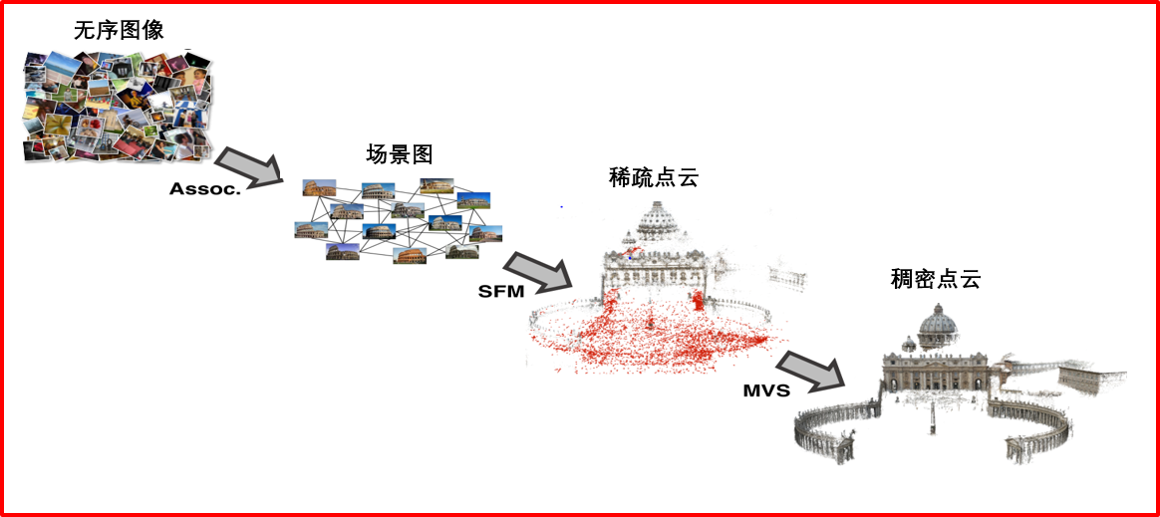
\includegraphics[width=10cm]{3Dconstr_pipiline_sfm.png}
    \caption{三维重建流程图}
    \label{fig:3Dconstr_pipiline_sfm}
\end{figure}
对于以上流程进一步进行细化,整个三维重建的过程可以划分为以下几个主要的步骤:

1.  2D图像采集:多角度拍摄或者从视频中提取到一组图像序列,将图像序列作为整个系统的输入;

2.  特征点提取和匹配:根据拍摄到的图像,提取每张图像之间的特征点,并进行特征点的匹配;

3.  稀疏点云:根据匹配结果估计特征点的深度,提取出稀疏点云,并估计相机的位姿和参数;

4.  稠密点云:根据优化后的相机参数和匹配结果,获得稠密点云;

5.  纹理映射:根据以上点重建物体表面,进行纹理映射。

三维重建的一般步骤可以简化为如图~\ref{fig:3Dconstr_pipiline}所示。
\begin{figure}[H] % use float package if you want it here
    \centering
    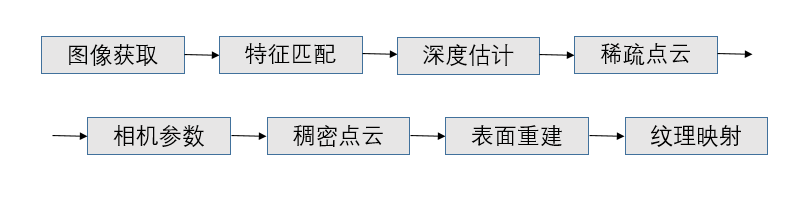
\includegraphics[width=10cm]{3Dconstr_pipiline.png}
    \caption{三维重建具体实现步骤图}
    \label{fig:3Dconstr_pipiline}
    \end{figure}
三维重建主要分为多个步骤,目前很多开源的系统都可以完成其中的部分环节,对于完整的三维重建流程还需要多个系统相互连接实现,表~\ref{tab:3D_compare}是当前三维重建系统的简要对比,其中绿色框图代表该重建系统包括该流程,灰色则不包括。
\begin{table}[h]
    \centering
    \caption{常见三维重建系统对比表}
    \label{tab:3D_compare}
    \begin{tabular}{C{3.6cm}C{2.4cm}C{2.4cm}C{2.4cm}C{2.4cm}}
    \toprule
    \textbf{系统名称} & \textbf{稀疏点云} &\textbf{稠密点云} &  \textbf{重建表面} &\textbf{纹理映射}  \\
    \midrule
    Bundler       &\cellcolor{green}是&\cellcolor{gray}否&\cellcolor{gray}否&\cellcolor{gray}否\\
    CMVS          &\cellcolor{gray}否&\cellcolor{green}是&\cellcolor{gray}否&\cellcolor{gray}否\\
    Colmap        &\cellcolor{green}是&\cellcolor{green}是&\cellcolor{green}是&\cellcolor{gray}否\\
    Meshlab       &\cellcolor{gray}否&\cellcolor{gray}否&\cellcolor{green}是&\cellcolor{green}是\\
    MVE           &\cellcolor{green}是&\cellcolor{green}是&\cellcolor{green}是&\cellcolor{gray}否\\
    MVS-texturing &\cellcolor{green}是&\cellcolor{green}是&\cellcolor{green}是&\cellcolor{gray}否\\
    openMVG       &\cellcolor{green}是&\cellcolor{green}是&否\cellcolor{gray}&\cellcolor{gray}否\\
    openMVS       &\cellcolor{gray}否&\cellcolor{gray}否&\cellcolor{green}是&\cellcolor{green}是\\
    Theia         &\cellcolor{green}是&\cellcolor{gray}否&\cellcolor{gray}否&\cellcolor{gray}否\\
    VisualFSM     &\cellcolor{green}是&\cellcolor{green}是&\cellcolor{gray}否&\cellcolor{gray}否\\
    \bottomrule
    \end{tabular}
  \end{table}
\subsection{三维重建详细过程解析}
\label{sec:3.2.2}
\subsubsection{图像获取} 
\label{sec:3.2.2.1}
目前三维重建仅需要输入无序图片,在构图的过程中,可以极大地降低操作的复杂度,并且对于相机的内参和外参也无需提前提供给整个三维重建的系统,在重建过程中,这些参数都可以计算得到。对于输入的图像,可以通过随着时间流单帧拍摄的方式获取或者通过截取视频流的方式得到,且图像之间不能仅有纯旋转,这样无法估计深度。对于堆体场景的图形采集,如图~\ref{fig:3Dconstr_get_picture}所示,需要注意保证每连续两帧图像之间尽可能保证30$\%$的重叠区域,相邻两帧之间的旋转角度为30度到45度之间,且物体中的每一个点至少能被三帧图像观测到。
\begin{figure}[h] % use float package if you want it here
  \centering
  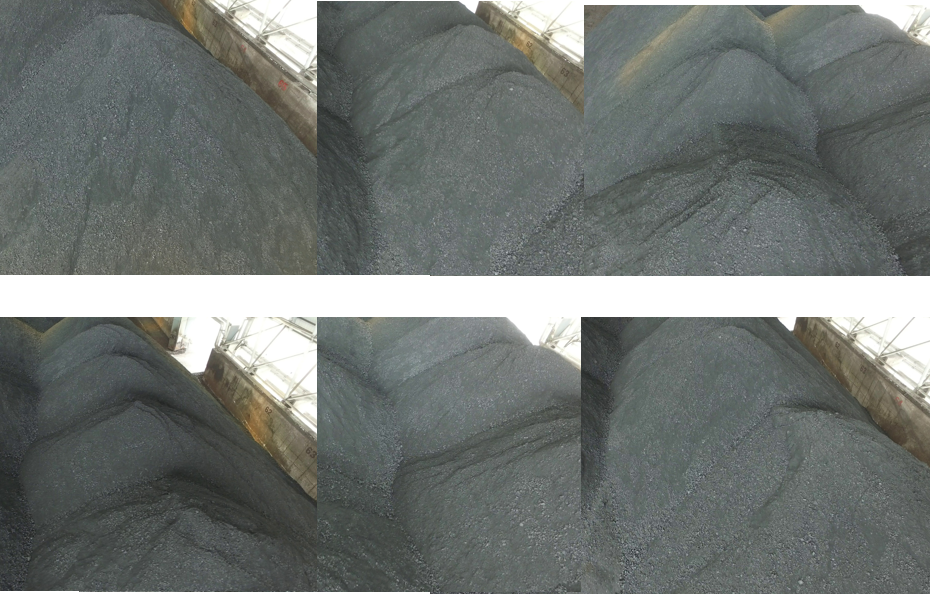
\includegraphics[width=10cm]{3Dconstr_get_picture.png}
  \caption{堆体图像采集示意图}
  \label{fig:3Dconstr_get_picture}
  \end{figure}
\subsubsection{特征点提取与检测} 
\label{sec:3.2.2.2}
特征是图像信息的另外一种数字表现形式,良好的特征应该是不受光线,噪音,几何变形影响的。目前,在三维重建领域中图像的特征匹配就是以特征点为基础而进行的,所以,如何定义和找出一幅图像中的特征点就非常重要,常见的特定点检测和匹配主要包括FAST,SIFT,ORB,Harris角点等。特征提取的目的是为了后续能够尽可能准确、稳定地估计出相机的运动,且特征点应该具备可重复性,高效率,可区别性以及本地性的特点,本文列举了在图像处理领域几种常用的特征检测和提取的方法。

\textbf{Harris角点:}当从不同的方向去移动一个视觉窗口,假设该区域内的灰度发生了很大的的变化,则认定存在角点。对于图像I(x,y),当在点(x,y)处平移(Δx,Δy)后的对应窗口的像素点灰度变化描述为:
\begin{equation}
  c(x, y ; \Delta x, \Delta y)=\sum_{(u, v) \in W(x, y)} (I(u, v)-I(u+\Delta x, v+\Delta y))^{2}
  \label{equ:Harris}
\end{equation}
结合泰勒分解公式,上式可以化简为:
\begin{equation}
  c(x, y ; \Delta x, \Delta y) \approx \sum_{w}\left(I_{x}(u, v) \Delta x+I_{y}(u, v) \Delta y\right)^{2}=[\Delta x, \Delta y] M(x, y)\left[\begin{array}{c}{\Delta x} \\ {\Delta y}\end{array}\right]
\end{equation}
其中
\begin{equation}
  \begin{split}
   & M(x, y)=\sum_{w}\left[\begin{array}{cc}{I_{x}(x, y)^{2}} & {I_{x}(x, y) I_{y}(x, y)} \\ {I_{x}(x, y) I_{y}(x, y)} & {I_{y}(x, y)^{2}}\end{array}\right]\\
   & =\left[\begin{array}{cc}{\sum_{w} I_{x}(x, y)^{2}} & {\sum_{w} I_{x}(x, y) I_{y}(x, y)} \\ {\sum_{w} I_{x}(x, y) I_{y}(x, y)} & {\sum_{w} I_{y}(x, y)^{2}}\end{array}\right] \\
   & =\left[\begin{array}{cc}{A} & {C} \\ {C} & {B}\end{array}\right] 
  \end{split}
  \end{equation}
公式~\ref{equ:Harris}即可转化为
\begin{equation}
  c(x, y ; \Delta x, \Delta y) \approx A \Delta x^{2}+2 C \Delta x \Delta y+B \Delta y^{2}
\end{equation}
又提出角度响应值R来判断该点是否为角点:
\begin{equation}
  R=\operatorname{det} \boldsymbol{M}-\alpha(\operatorname{trace} \boldsymbol{M})^{2}
\end{equation}
通过以上公式可以看出,Harris角点具备以下特点:

1. 对亮度和对比度的变化不敏感:因为微分运算对图像密度的变化不敏感,即亮度或者对比度的变化对Harris的检出影响较小;

2. 具有旋转不变性:Harris角点检测算子的本质可以表示为一个椭圆,但椭圆旋转时,并不会影响R值的大小;

3. 不具有尺度不变性。

\textbf{FAST特征点:}对图像中的中的一个像素p,假设其亮度值为$I_p$,阈值为t,如图所示,取以其为中心,半径为是三个像素的圆,圆上共有16个像素点,假设这16个点中有连续N个点都比$I_p+t$大或者比$I_p-t$小,则认定其为Fast角点,如图~\ref{fig:3Dconstr_Fast}所示,为了加快检测过程,会直接检测第1,5,9,13这4个点,如果有三个满足要求,也会认为是角点。
\begin{figure}[H] % use float package if you want it here
  \centering
  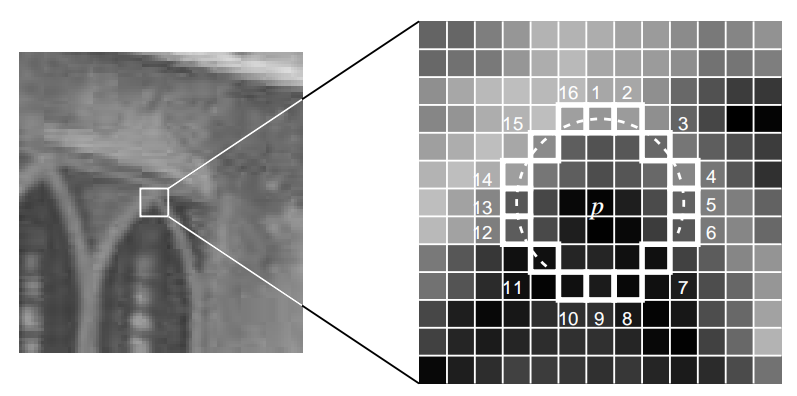
\includegraphics[height=4.5cm]{3Dconstr_Fast.png}
  \caption{FAST特征点}
  \label{fig:3Dconstr_Fast}
\end{figure}
\textbf{ORB特征点:}结合了FAST特征点的检测和BRIEF描述子,其中RIEF特征描述符的计算过程:首先平滑图像,在某个像素点的周围选择一个领域,根据特定的点对选择方法挑选出$n_d$个点对,比较每个点对之间亮度值的大小,即可得到一个长度为$n_d$的二进制串。由于FAST特征点不具有方向,ORB在此基础上进行了改良,即利用灰度质心法求解出灰度额质心之间的偏移方向,首先定义特征点p的邻域像素的矩:
\begin{equation}
  m_{p q}=\sum_{x, y} x^{p} y^{q} I(x, y)
\end{equation}
图像的质心为:
\begin{equation}
  C=\left(\frac{m_{10}}{m_{00}}, \frac{m_{01}}{m_{00}}\right)
\end{equation}
那么偏移方向可以定义为FAST的特征点方向:
\begin{equation}
  \theta=\arctan \left(m_{01}, m_{10}\right)
\end{equation}

以上说明了图像处理中常用的特征点提取方式,如图~\ref{fig:3Dconstr_a}和~\ref{fig:3Dconstr_b}先分别对两张堆体图像进行特征提取。接下来将以此为基础说明特征点的匹配过程:在获取到每张图像上的特征点后,需要对图像之间建立匹配关系,常用的方式可以采用计算欧式距离的办法:

1. 完全匹配,对所有的特征点都进行穷举,计算其对应距离。

2. 邻近搜索,建立KD树,缩小搜索范围,能提高效率,但也有可能不是最优,所以邻域取值是关键,越大越准确,越大计算量越大。

如图~\ref{fig:3Dconstr_match}所示,两帧之间大多数特征点都可以正确匹配,但依然存在存在部分匹配是错误的,在本文中,选择了RANSAC(随机抽样一致性)的方式来剔除错误的匹配对,以更加准确的估计相机位姿,RANSAC是指可以从一组包括局外点(错误匹配)的观测数据中,通过迭代的方式估计数学模式中的参数,通过RANSAC处理后的匹配结果如图~\ref{fig:3Dconstr_matchAfterRansac}所示,误检的匹配已经被明显的降低。
\begin{figure}[H]
    \centering
      \subcaptionbox{第1帧图像特征提取\label{fig:3Dconstr_a}}{
      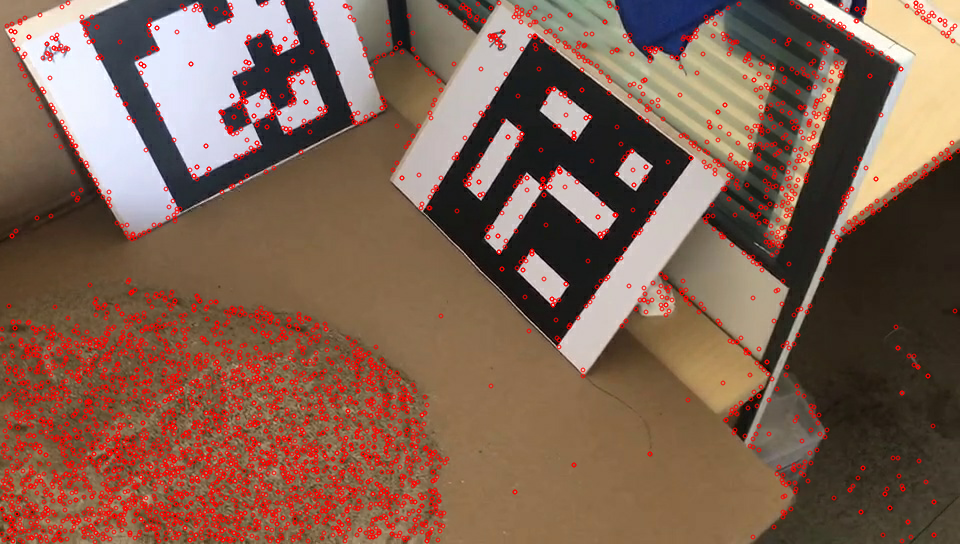
\includegraphics[width=4.5cm]{3Dconstr_a.png}}
      \subcaptionbox{第2帧图像特征提取\label{fig:3Dconstr_b}}{
      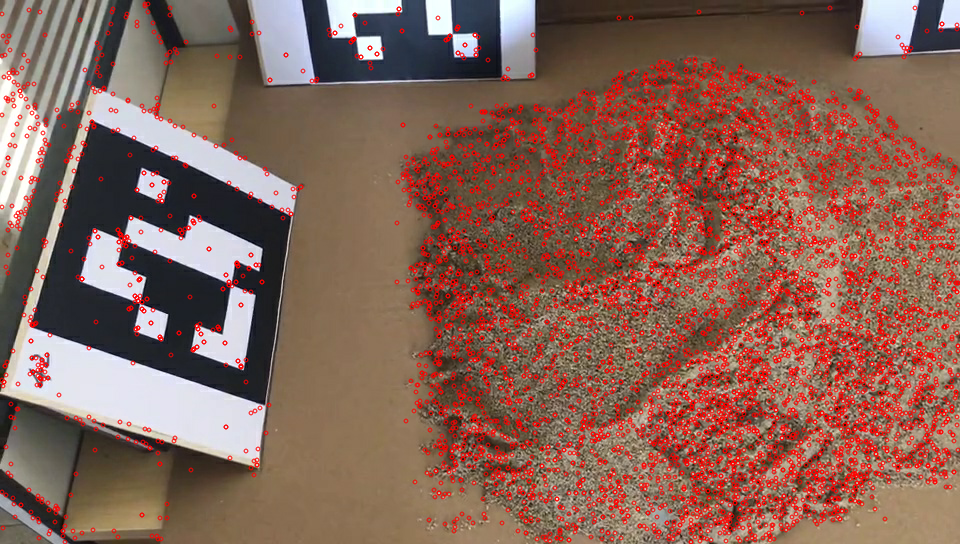
\includegraphics[width=4.5cm]{3Dconstr_b.png}}
    \vskip0.5cm
      \subcaptionbox{特征点匹配示意图\label{fig:3Dconstr_match}}{
      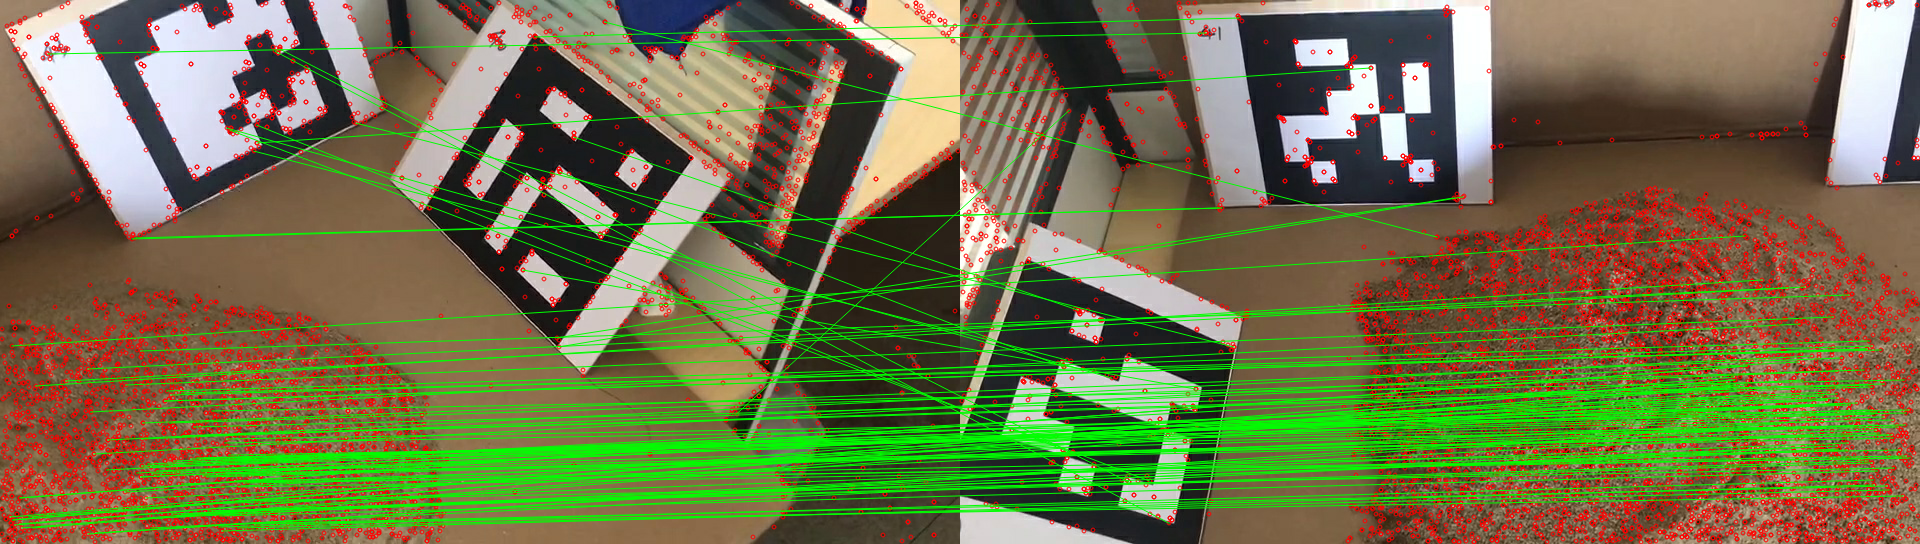
\includegraphics[width=10cm]{3Dconstr_match.png}}
    \vskip0.5cm
      \subcaptionbox{RANSAC后的特征匹配示意图\label{fig:3Dconstr_matchAfterRansac}}{
      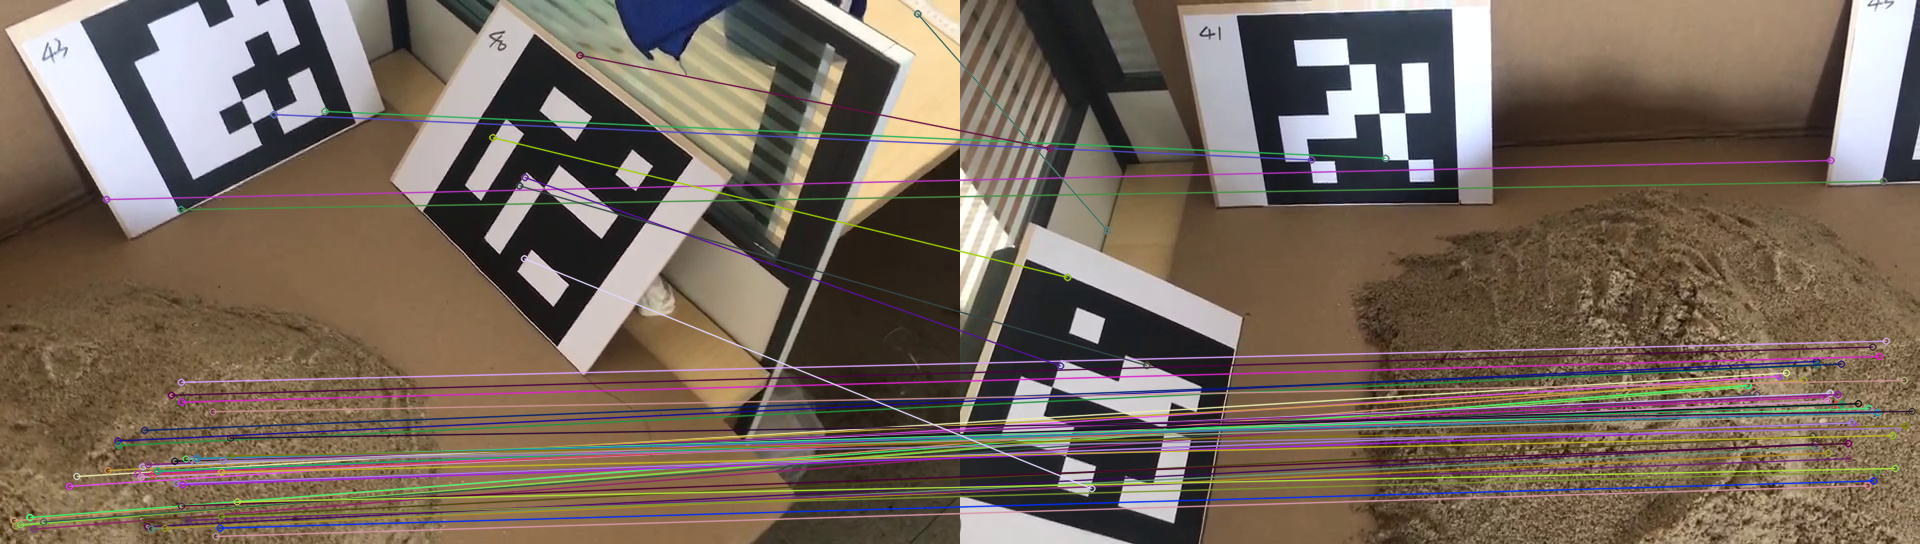
\includegraphics[width=10cm]{3Dconstr_matchAfterRansac.png}}
    \caption{特征提取与匹配结果示意图}
    \label{fig:3Dconstrmatch}
\end{figure}
\subsubsection{SfM} 
\label{sec:3.2.2.3}
在~\ref{sec:3.2.2.2}小节中,可以获得初始的匹配关系,但是这种匹配关系不完全可靠,需要添加几何约束进行检测,该集合约束完全依赖于场景中的客观事实。可以通过基本矩阵F将匹配好的两帧图像之间的像素坐标(x,y),(x',y')进行关联,假设一个符合条件的匹配对像素坐标需要满足以下公式:
\begin{equation}
\begin{bmatrix}x'&y'&z'\end{bmatrix}\mathrm F\begin{bmatrix}\mathrm x\\\mathrm y\\\mathrm z\end{bmatrix}=0
\end{equation}

找到相机基线最大的像对,根据该像对,通过RANSC八点法计算本征矩阵,再通过对本征矩阵SVD分解得到第二个图像的R、T,在这一步需要进行畸变校正,然后根据R、T和矫正后的像点坐标三角计算出三维点。
当所有的两两匹配图像对被确定以后,可以开始计算相机的位姿(3*3的旋转矩阵R,1*3的平移向量t),摄像机的内参(焦距f,畸变参数$k_1$,$k_2$)。几何场景提供轨迹中的每个3D点$X_j$,通过投影方程,将3D点投影到摄像机的2D成像平面上,投影误差的定义为投影点和图像上真实点之间的欧式距离,如图~\ref{fig:3Dconstr_reprojection-error}所示。
\begin{figure}[H] % use float package if you want it here
  \centering
  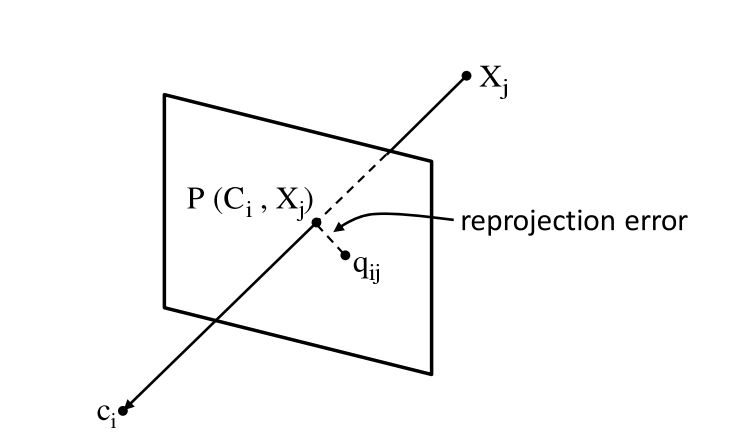
\includegraphics[width=5cm]{3Dconstr_reprojection-error.png}
  \caption{误差投影示意图}
  \label{fig:3Dconstr_reprojection-error}
\end{figure}
对于n个视角和m个轨迹,投影误差的目标优化方程为:
\begin{equation}
  \mathfrak g(C,X)=\sum_{i=1}^n\sum_{j=1}^m\omega_{ij}\left|\left|q_{ij}-P(C_i,X_j)\right|\right|^2
\end{equation}
其中$\left|\left|q_{ij}-P(C_i,X_j)\right|\right|^2$就是摄像机i中的轨迹j的投影误差累积和,SFM算法的目标就是找到合适的相机和场景参数去优化这个目标函数,g是采用一个非线性最小二乘的优化方法求解,常用BA(光束平差法)来优化上述过程。最后,不断添加新的摄像机和3D点进行BA。这个过程直到剩下的摄像机观察到的点不超过20为止,说明剩下的摄像机没有足够的点可以添加,BA结束。得到相机估计参数和场景几何信息,即稀疏的3D点云。
\subsubsection{MVS} 
\label{sec:3.2.2.4}
SfM是指从运动中恢复结构的过程,而MVS则是多视角立体视觉生成统,SfM生成的是稀疏点云,恢复相机之间的几何关系,MVS生成的是稠密点云,由SfM获得的一些相机参数和相机之间的几何关系,来进行MVS。在SfM中,重建的点都是由特征匹配的点,这些点集本身就就不稠密,因此无法获取到稠密的点云,而在三维重建的过程就需要通过MVS的方式获取稠密的点集,MVS利用图像中的像素点来实现点云的重建,将图像中的每一个像素点估计其三维坐标,构成稠密点云。

在稠密点云的估计过程中,无法将每一个像素点按照特征点的方式计算其描述子,因此提出了极线搜索和快匹配技术来匹配图像中的某一像素点在其他图像中的对应的点,在找到每一个像素点在其他图像中出现的位置之后,就可以利用三角测量的发放确定其深度,但是因为用一个像素点会出现在多个图像中,所以就期望通过多次三角化让该点的深度值收敛。

对于极线搜索和块匹配技术,如图~\ref{fig:3Dconstr_jixiansousuo}所示。
\begin{figure}[H] % use float package if you want it here
  \centering
  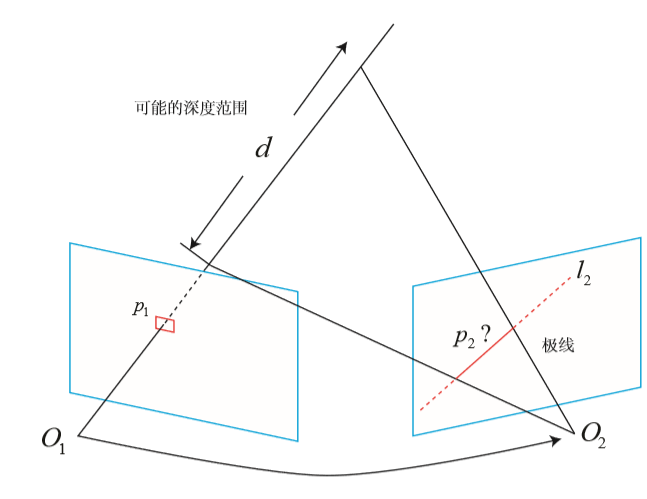
\includegraphics[width=5cm]{3Dconstr_jixiansousuo.png}
  \caption{极线搜索示意图}
  \label{fig:3Dconstr_jixiansousuo}
\end{figure}
首先对于极线搜索和块匹配技术,如图所示,左侧的相机观测到了像素点$p_1$,由于该相机为单目相机,没法确定深度,可以先假设该点的实际位置在0到正无穷的区间中,因此该像素对应的空间点就分布在某条线段上,对于右侧相机,上述线段可以在成像平面上生成一段投影,在已知两帧图像之间的相对位姿时,是可以确定该极线的位置的,接下来就需要在极线上寻找与像素点$p_1$所对应的$p_2$点的位置。

因为单个像素没有对应的特征值,无法进行匹配,此外依靠单个特征点的亮度来进行匹配也并不可靠,可以基于图像块在前后变化得到过程中的灰度不变性特征,在P1周围选育一块w*w得到小块,然后在右侧的极线上选择多个这样的小块来提高区分度。对于计算两个小块之间的差异,一般可以通过以下方法来计算:

1.SAD取两个小块的差的绝对值之和
\begin{equation}
  S{(A,B)}_{SAD}=\sum_{i,j}\left|A(i,j)-B(i,j)\right|
\end{equation}
2.SSD取两个小块比较求平方和
\begin{equation}
S{(A,B)}_{SSD}=\sum_{i,j}(A(i,j)-B{(i,j))}^2
\end{equation}
3.NCC取两个小块计算相似性
\begin{equation}
  S{(A,B)}_{NCC}=\frac{{\displaystyle\sum_{i,j}}A(i,j)B(i,j)}{\sqrt{{\displaystyle\sum_{i,j}}A{(i,j)}^2\underset{i,j}\sum B{(i,j)}^2}}
\end{equation}
在极线上,计算了 A 与每一个 Bi 的相似性yo度量,那么将得到一个沿着极线的数值分布,该分布的形状取决于图像本身信息,在搜索距离较长的情况下,通常会得到一个非凸函数:该分布存在许多峰值,但是真实值只有一个,接下来需要使用深度滤波器使用概率分布来描述深度值从而找到对应的$p_2$点。

根据以上流程,可以对图~\ref{fig:2VSLAM_big}所示的连续堆体图像进行三维重建,堆体点云重建结果如图~\ref{fig:3dconstr_sparse}所示。
\begin{figure}[H]
  \centering
    \subcaptionbox{稀疏重建示意图\label{fig:3Dconstr_match}}{
    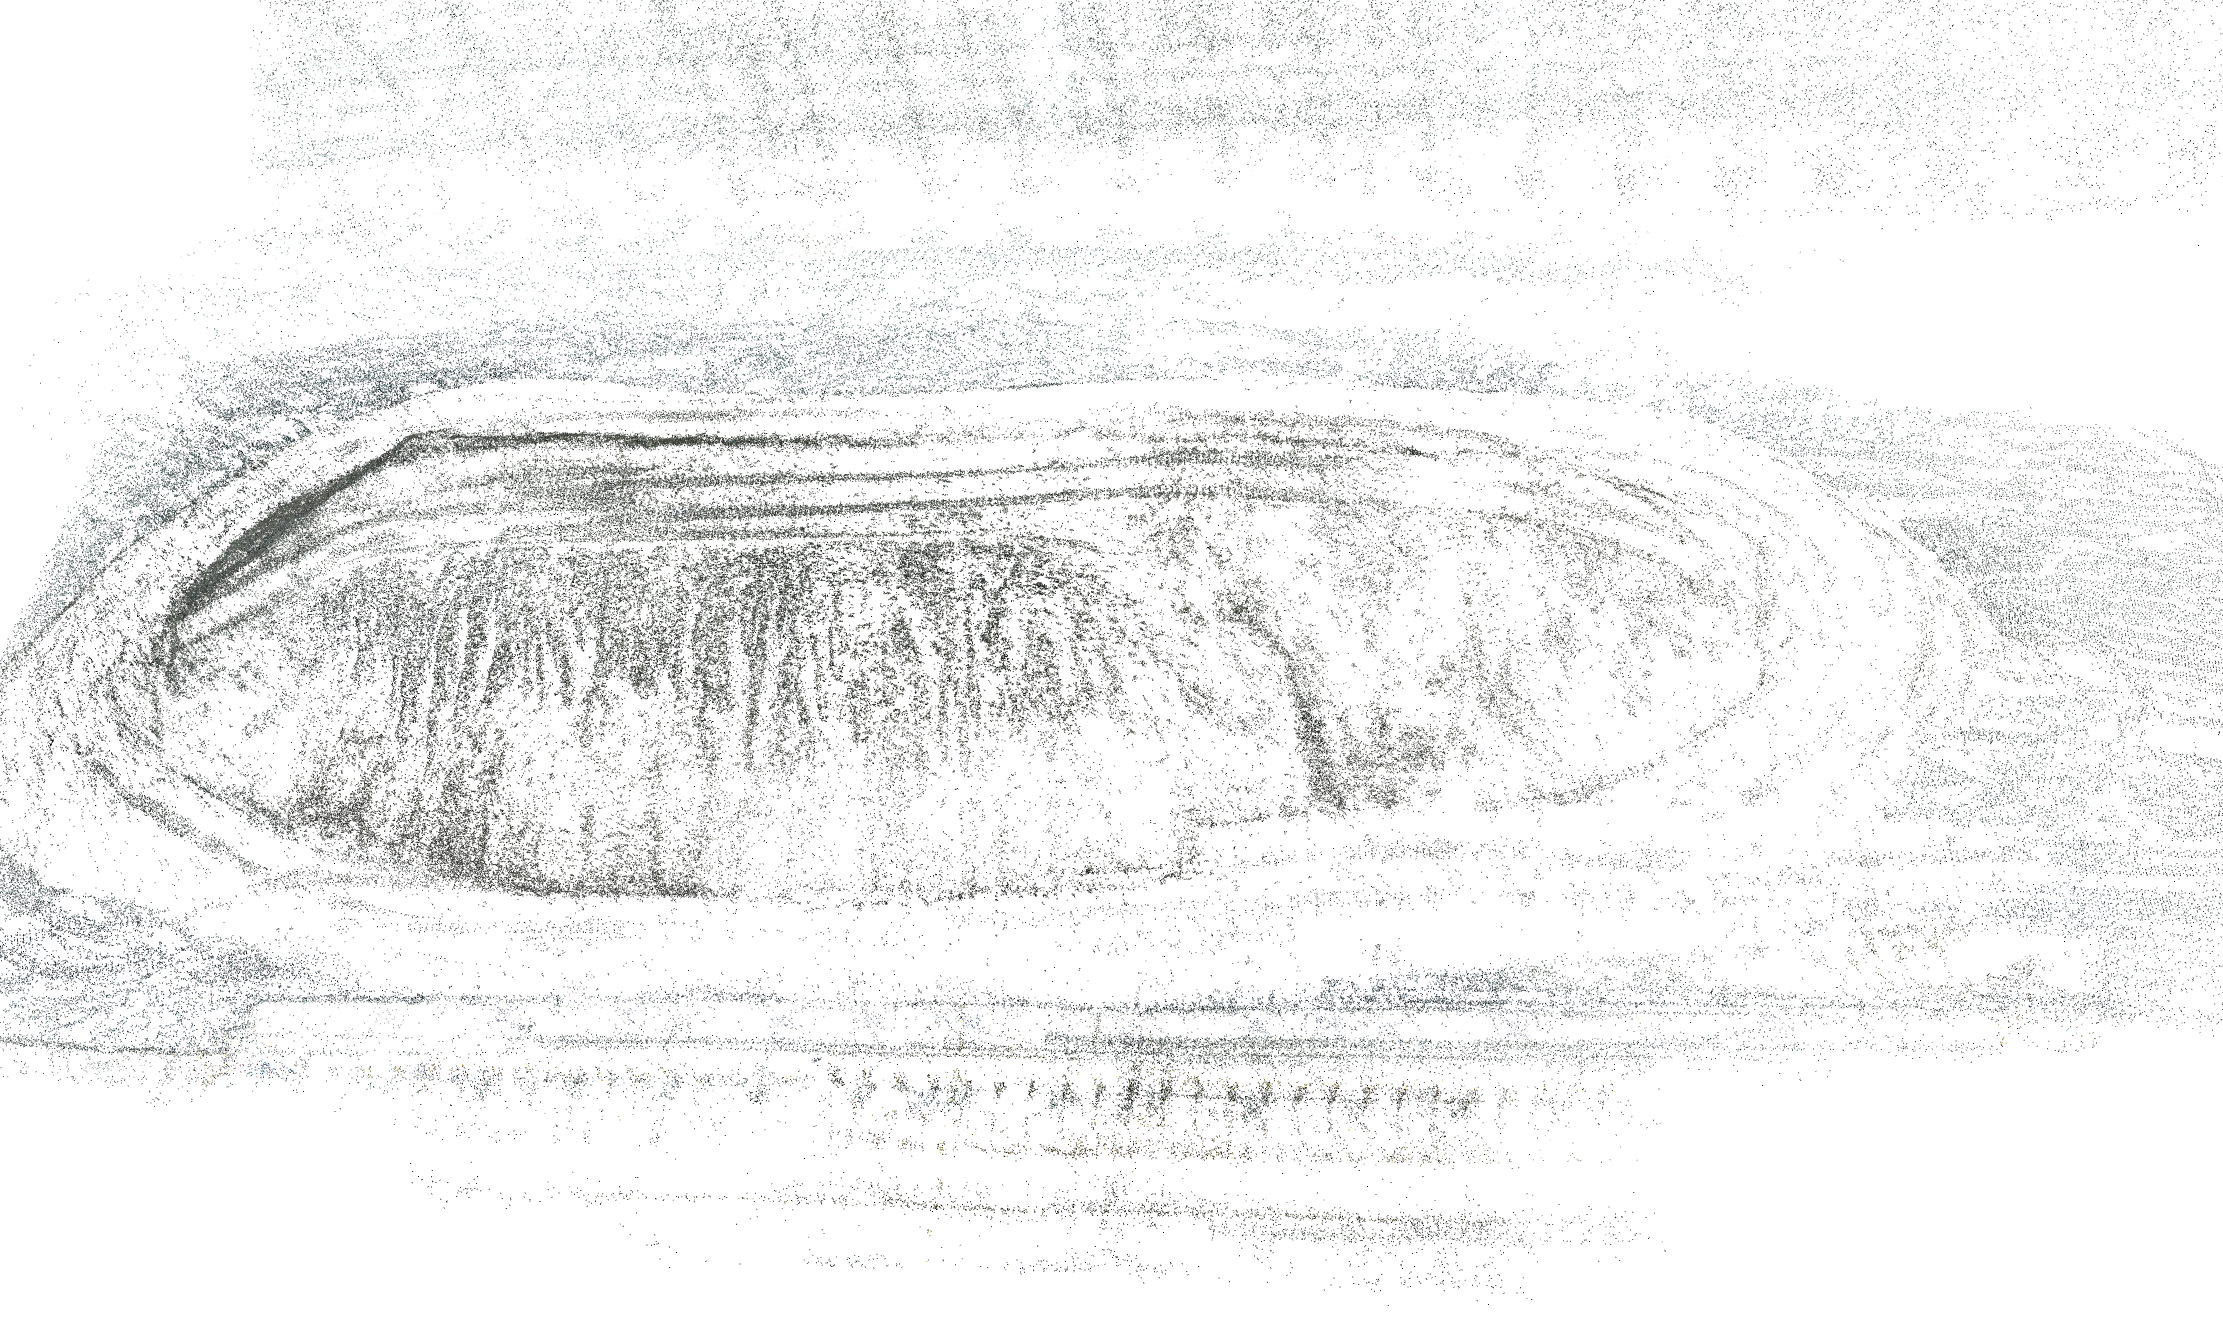
\includegraphics[width=12cm,height=5cm]{3dconstr_sparse.png}}
  \vskip0.5cm
    \subcaptionbox{稠密重建示意图\label{fig:3Dconstr_matchAfterRansac}}{
    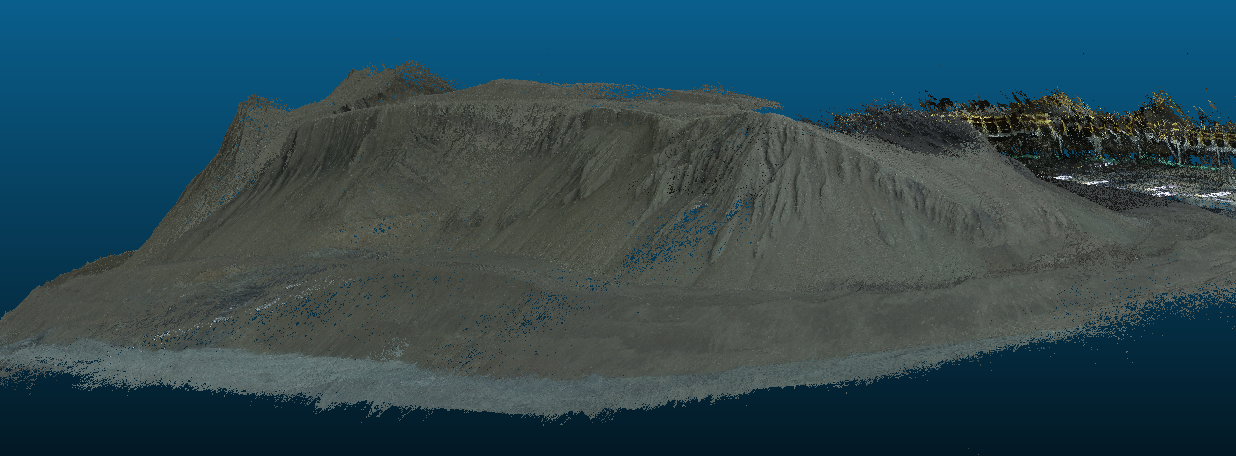
\includegraphics[width=12cm,height=5cm]{3dconstr_dense.png}}
  \caption{堆体稀疏重建和稠密重建示意图}
  \label{fig:3dconstr_sparse}
\end{figure}
\subsection{当前三维重建存在的问题}
\label{sec:3.2.3}
根据~\ref{sec:3.2.2}节的描述,可以发现通过现有的三维重建技术流程可以实现对多张连续图像到三维点云的转化,整个过程操简便,且能够得到一个较好的结果。但是从整体耗时情况,三维点云结果的精确性来看,依然还存在以下问题:

1. 整个三维重建的过程十分耗时,由于三维重建中的图像输入没有时序信息,关键帧之间的匹配通过完全枚举的方式进行,当输入N张原始图像时,系统的时间复杂度高达O($N^2$),由单帧图像到稀疏点云一般耗时为几分钟,由单帧图像到稠密点云耗时耗时更是会高度几个小时。

2. 三维点云的精度不高,噪音点较大,一方面是由于三维重建往往采取增量式的重建方式,导致最终场景重建的结果无法闭合;另外一方面由于对于某些重复度较高的场景,关联帧之间的匹配由于缺少时序信息,从而导致匹配精度较低,在解算相机位姿时,得到的结果也无法保证正确,如图~\ref{fig:3dconstr_stone}所示。
\begin{figure}[h]
  \centering
    \subcaptionbox{正面}{\label{fig:chap1:3dconstr_stone1}
    \includegraphics[width=3.5cm,height=4.5cm]{3dconstr_stone1.JPG}}
    \subcaptionbox{斜侧面}{\label{fig:chap1:3dconstr_stone2}
    \includegraphics[width=3.5cm,height=4.5cm]{3dconstr_stone2.JPG}}
    \subcaptionbox{侧面}{\label{fig:chap1:3dconstr_stone3}
    \includegraphics[width=3.5cm,height=4.5cm]{3dconstr_stone3.JPG}}
  \vskip0.5cm
  \subcaptionbox{无法闭合}{\label{fig:chap1:3Dconstr_stone1}
  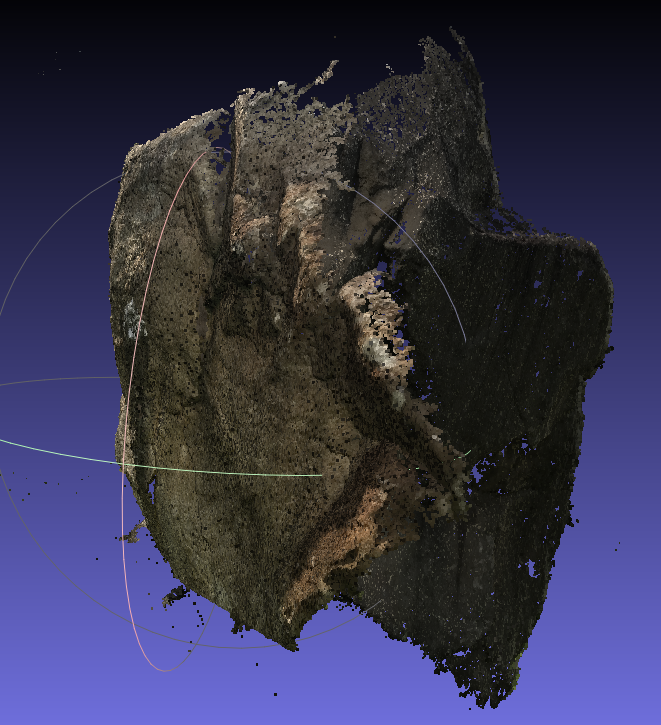
\includegraphics[width=3.5cm,height=4.5cm]{3Dconstr_stone1.png}}
  \subcaptionbox{缺失较多}{\label{fig:chap1:3Dconstr_stone2}
  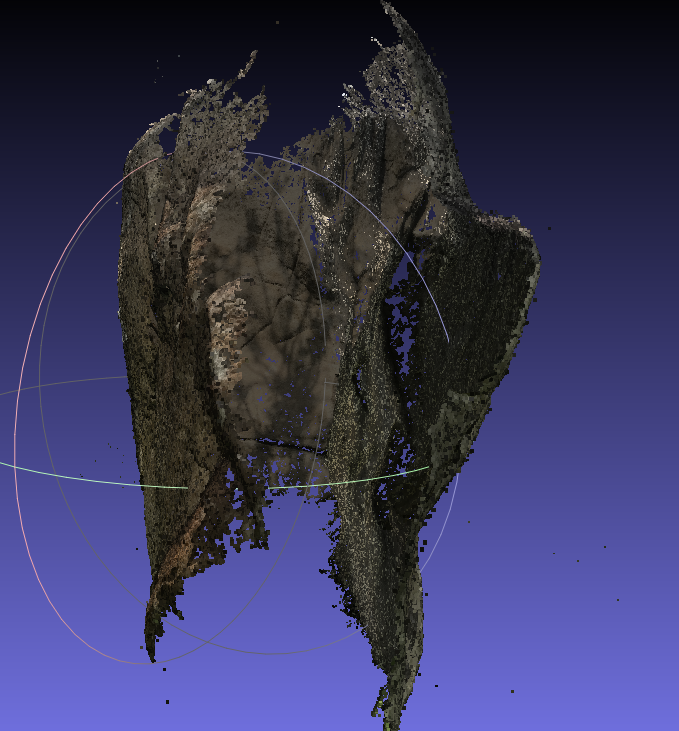
\includegraphics[width=3.5cm,height=4.5cm]{3Dconstr_stone2.png}}
  \subcaptionbox{噪音点多}{\label{fig:chap1:3Dconstr_stone3}
  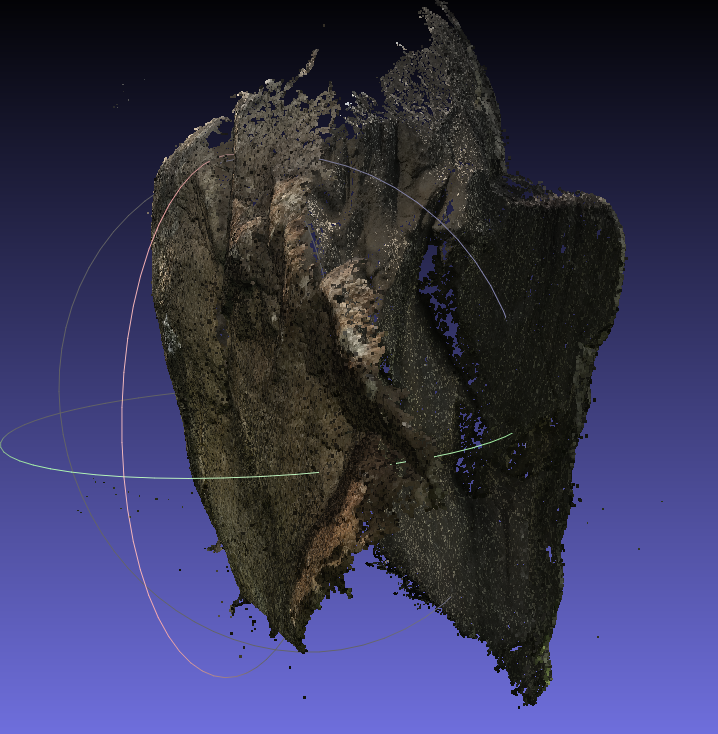
\includegraphics[width=3.5cm,height=4.5cm]{3Dconstr_stone3.png}}
  \caption{自然场景三维重建结果示意图}\label{fig:3dconstr_stone}
\end{figure} 
\section{三维重建优化方案研究}
\label{sec:3.3}
% \subsection{解决贫纹理方案}
% \label{sec:3.3.1}
% 对于一些常见的工业工件,多由金属构成,表面光滑无显著纹理信息,如图~\ref{fig:3Dconstr_iron1}所示,在特征提取环节难以提取到特
% 征对,对于后续的匹配和三角化过程都难以进行,且在以光源下,存在很严重的反光问题,对于不同视角下会生成不同的图像信息影响建模。
% 因此现在提出一种在金属器件表面涂上荧光剂的方法来改良贫纹理工件难以三维建模的问题,如图~\ref{fig:3Dconstr_iron2}所示。
% \begin{figure}[H]
%   \centering%
%   \subcaptionbox{金属工件原图\label{fig:3Dconstr_iron1}}{%    
%     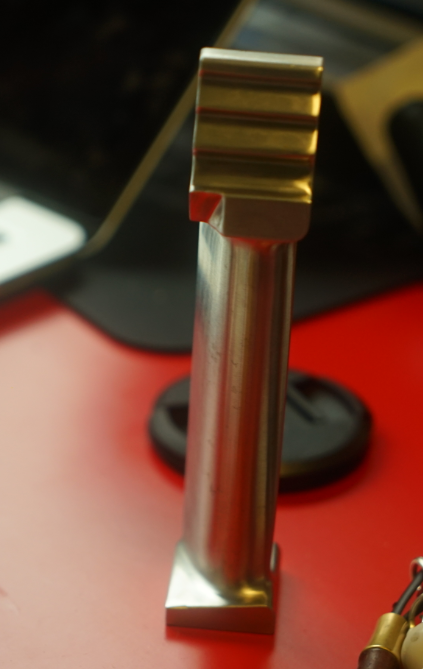
\includegraphics[height=6cm]{3Dconstr_iron1.png}}\hspace{2em}%
%   \subcaptionbox{金属工件添加荧光剂示意图\label{fig:3Dconstr_iron2}}{%    
%     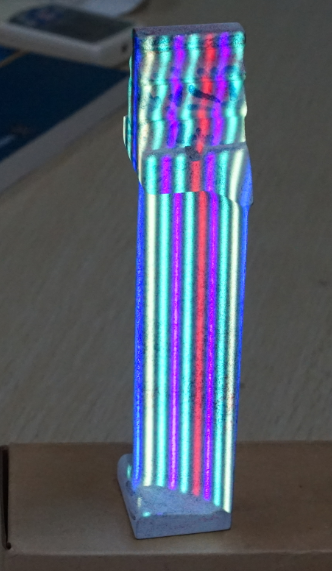
\includegraphics[height=6cm]{3Dconstr_iron2.png}}
%   \caption{金属工件示意图}
%   \label{fig:3Dconstr_iron}
% \end{figure}
% 按照~\ref{sec:3.2}节的流程,可以获得如图~\ref{fig:3Dconstr_iron3}所示的三维点云结果图。
% \begin{figure}[H] % use float package if you want it here
%   \centering
%   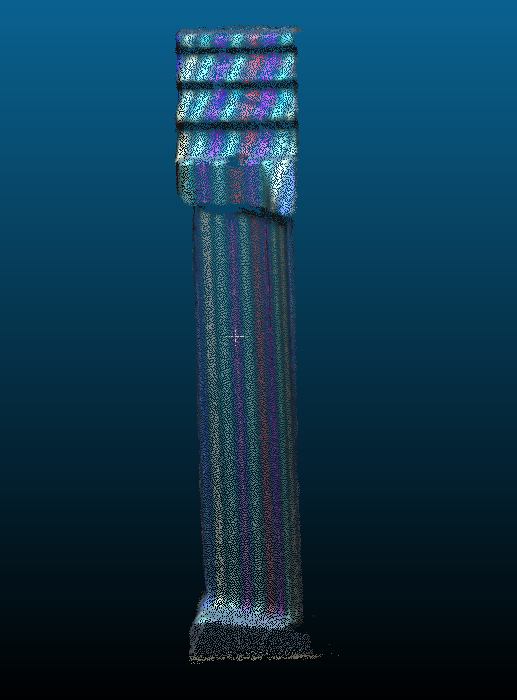
\includegraphics[height=9cm]{3Dconstr_iron3.png}
%   \caption{金属工件三维重建结果示意图}
%   \label{fig:3Dconstr_iron3}
% \end{figure}
\subsection{增加实效性方案}
\label{sec:3.3.2}对无序的图像进行三维重建时,会有大量的时间耗费在图像的匹配过程中,在三维重建中常见的图像匹配方法包含以下几种模式:

1. 完全匹配:适用于三维重建的图像数量较低时,这种匹配模式一般可以较快的完成,并且产生一个比较好的匹配结果,在这种模式里,每一帧图像都会和其他所有的图像进行匹配验证。但是一旦图像的数量较大,那么这种图形匹配方式将极其耗时,延缓整个三维重建的实效性。

2. 序列匹配:一般用于图像帧连续获取的情况下,存在视觉重叠部分,这样就不需要对所有帧进行完全匹配,只需要考虑前后帧即可。

3. 空间匹配:考虑每一帧图像的空间位置,通过空间位置获取到和其相邻的匹配帧,每一帧的空间位置可以通过图像自带的GPS信息获取,该模式对提供的图像空间位置精度要求较高。

4. 传递匹配:当确定帧A和帧B都和帧C有匹配关系时,那么就默认帧A和帧B也具备匹配关系,这样的匹配模式实效性较快,但是误差较大。

5. 自定义匹配:即在系统进行匹配查找时,就将所有的匹配关系自定义给出,以自定义的匹配结果代替三维重建中的匹配方法。

对于上述几种匹配模式,需要同时考虑到匹配时效和匹配精度的问题。排除空间匹配的方法,因为在密闭的环境中很难获取到每一帧图像对应的真实GPS信息,图像所自带的EXIF信息也会受到GPS强弱的影响,此外通过无人机获取到得到图像,即使有两帧之间的空间位置十分接近,也无法保证两帧图像具备匹配关系,例如在无人机正反来回的的两帧即使空间位置十分接近,也不一定是匹配帧。

对于自定义的匹配模式,本文将以SLAM的结果提供给三维重建进行图像匹配,即以有序化的图像输入代替无序化的图像输入,一方面可以避免完全匹配带来的耗时问题,同时具备时序信息的SLAM所产生的匹配结果更加精确。对于具体的实现过程,以连续视频流作为SLAM系统的输入,筛选出其中的关键帧和所有关键帧之间的对应关系,将SLAM中的关键帧作为三维重建的图像输入,关键帧之间的匹配关系作为三维重建的先验匹配结果,具体流程如图~\ref{fig:3Dconstr_SLAM_pipeline}所示。
\begin{figure}[h] % use float package if you want it here
  \centering
  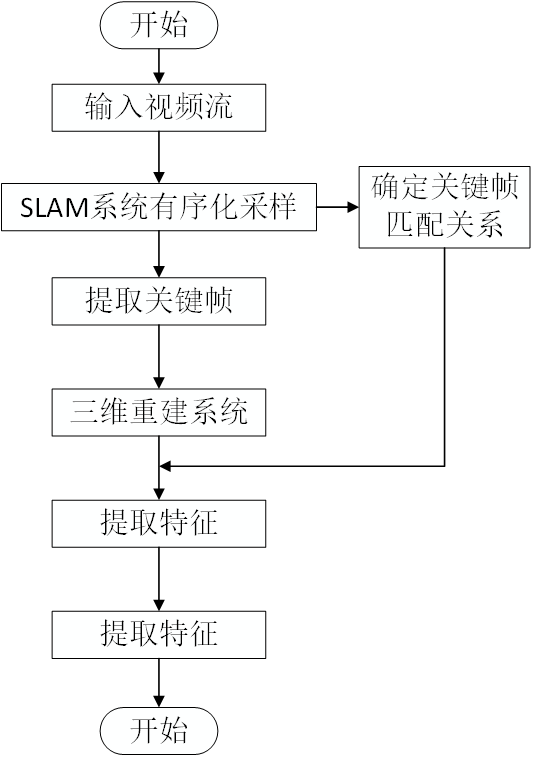
\includegraphics[height=9cm]{3Dconstr_SLAM_pipeline.png}
  \caption{融合SLAM结果的三维重建流程图}
  \label{fig:3Dconstr_SLAM_pipeline}
\end{figure}

以下将讨论SLAM中关键帧的提取和匹配策略。关键帧相当于SLAM的框架,是在局部一系列普通帧中选出一帧作为局部帧的代表,记录局部信息,但相机在场景中的某个区域内移动时,普通帧的集合会不断增减,导致连续的两个普通帧之间会存在大量的信息冗余,如果所有普通帧全部参与计算,就会极大的浪费算力和内存, 因此为了保证整个SLAM系统的良好运行,都会选择关键帧来作为优化对象。此外,关键帧选择时还会对图片质量、特征点质量等进行考察,一定程度上也发挥了滤波的作用,防止无用的或错误的信息进入优化过程而破坏定位建图的准确性。

选择关键帧主要从关键帧自身和关键帧与其他关键帧的关系两个方面来考虑。一方面,关键帧自身质量要好,例如不能是非常模糊的图像、特征点数量要充足、特征点分布要尽量均匀等等;另一方面,关键帧与其他关键帧之间的关系,需要和局部地图中的其他关键帧有少量的共视关系,但大部分特征点是新特征点,以达到既存在约束,又尽量少的信息冗余的效果,例如局部地图点投影到此帧的点数低于一个阈值或前一个关键帧的特征点在此帧里已经有90$\%$观测不到等等。对于关键帧的选择,一般有以下策略:

1. 距离上一关键帧的帧数是否足够多,主要从间隔的时间上来考虑,例如可以直接间隔固定帧数选择一个关键帧,这样操作流程简单,但是整体取帧效果不好,因为对于一些运动缓慢的场景,会选择大量相似的关键帧,再次造成冗余的情况,在运动较快的场景,又容易造成大量有效帧的缺失。

2. 距离上一关键帧的距离是否足够远,主要从空间位置上来考虑,在SLAM运行的过程中,可以根据相机位姿得到帧和帧之间的位置关系,如果运动的距离足够大,那么可以直接将其确定为下一个关键帧,但在对某一个场景进行重复来回运动时,就会收集大量重复的关键帧。

3. 跟踪质量,主要从共视特征点上来考虑,在SLAM的过程中会记录下当前视角中的信息,一旦检测到离开当前视角则加入新的关键帧,和上两种方法相比较能够更有效的获取到关键帧。

对于本文中三维重建图像输入的选择,优先选择第三种关键帧提取方案,避免了提取帧率过小,而丢失一些三维重建时关键的帧,提取帧率过大而造成图片集合存在大量冗余的问题。此外通过SLAM的筛选策略也可以提前过滤掉存在运动模糊和质量过低的图像。
\subsection{增加精确性方案讨论}
\label{sec:3.3.3}
针对~\ref{sec:3.2.3}节所提出的问题,本文提出一种结合SLAM结果的三维重建方法,包括SLAM生成的KeyFrame DataBase以及位姿信息,以提高点云结果的鲁棒性和准确性。本文所提出的建图过程分为两个阶段:在线SLAM阶段和离线3D重建阶段。

在线SLAM阶段实时获取单目相机的图像信息,结合SLAM技术快速建立scene graph及点云环境地图。由于在线SLAM注重实时性能,只是对局部窗口进行增量优化,即使在闭环时也只进行轨迹和部分点云优化,可以动态获取KeyFrame DataBase和较为准确的位姿信息。所建立的scene graph及点云环境地图的精度较低。随着时间的推移不可避免的会出现误差累计,导致闭环处出现轨迹和环境地图的断口问题。

离线3D重建阶段首先基于在线SLAM阶段所建立的粗糙scene graph及点云环境地图,以大尺度地图及运动轨迹为优化目标,利用高性能计算机的快速处理能力进行全局优化,得到更加精确的全局稀疏地图和运动轨迹;然后基于MVS技术建立稠密/半稠密环境地图。下面分别详细说明在线SLAM过程和离线3D重建过程。
\subsubsection{在线SLAM阶段}
\label{sec:3.3.3.1}
本文所提出的SLAM系统整体框架如图~\ref{fig:3d_constr_online_SLAM.png}所示。系统的输入为单目相机(内参标定结果已知)。SLAM系统有前端-后端两个部分构成,前端进行特征提取及数据关联,后端进行图模型建模及Maximum a Posteriori优化。
\begin{figure}[h] % use float package if you want it here
  \centering
  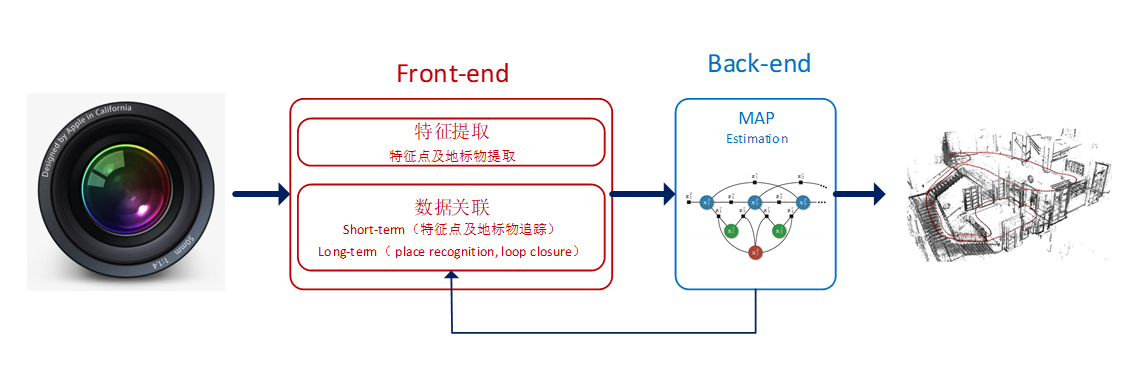
\includegraphics[height=4.5cm]{3d_constr_online_SLAM.png}
  \caption{前视SLAM整体框架}
  \label{fig:3d_constr_online_SLAM.png}
\end{figure}
当前主流vSLAM通过多线程技术维护3个模块,实现前端-后端的各项功能,如图~\ref{fig:3d_constr_SLAM}所示。系统以地图数据为核心,以BA图模型优化为手段,实现了相机追踪、地图维护、闭环优化。
\begin{figure}[h] % use float package if you want it here
  \centering
  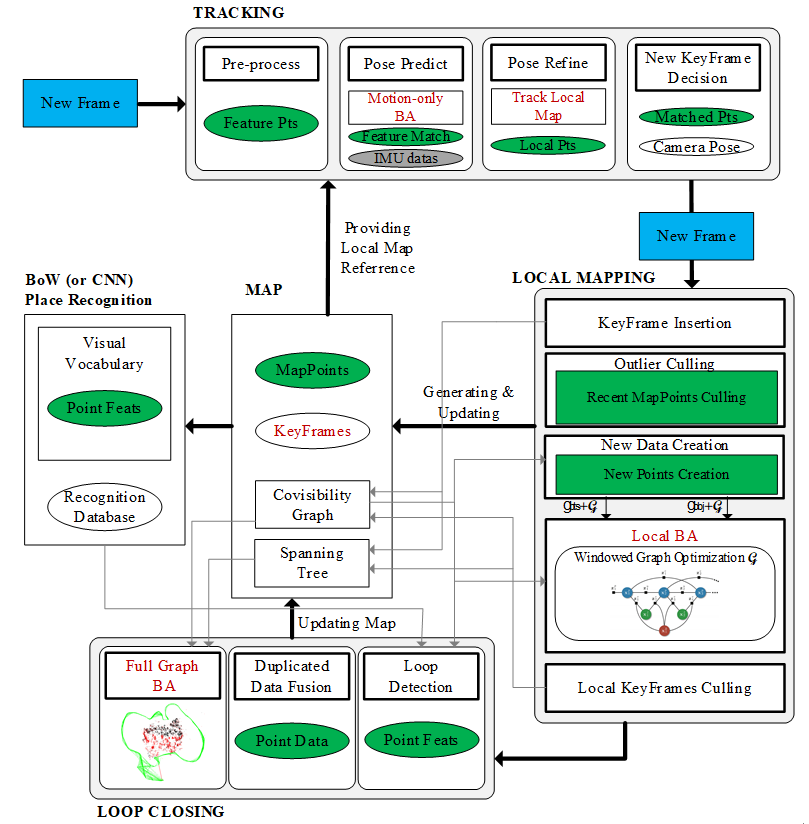
\includegraphics[height=9cm]{3d_constr_SLAM.png}
  \caption{SLAM系统框架图}
  \label{fig:3d_constr_SLAM}
\end{figure}
图中绿色模块代表传统点特征数据,通过特征提取、数据关联、地图维护、词袋维护,闭环检测等流程被不断的加入到factor graph中并进行优化估计。

\textbf{追踪:}模块主要负责计算相机在这两帧之间的相对运动,通过相机姿态累计得到相机的运动轨迹。首先通过图像预处理提取点特征及语义地标特征,基于两帧间特征匹配利用Motion-only BA进行运动姿态估计,基于图像特征与地图数据关联结果利用闭环进行姿态优化,最后通过计算当前帧的信息增量的多少判别其如果是关键帧则将其输送给地图构建模块。

\textbf{地图构建:}模块将追踪模块新输送过来的关键帧数据与已有关键帧数据根据可共视性约束进行数据匹配,在factor graph图模型中加入新的点特征节点并完成数据关联,根据可共视性约束确定局部优化范围,通过Local Mapping BA建立并优化地图数据。

\textbf{闭环:}模块通过检测匹配环境地标以判断相机是否再次运动到之前曾经到过的区域,并根据这一信息对相机的运动轨迹及地图数据进行全局修正,降低累积误差。本项目拟基于BoW词袋技术进行闭环检测。在闭环修正时时首先对地图中的重复点特征进行融合,然后对闭环主干网络进行全局BA,实现轨迹和地图数据的正确闭环。
\subsubsection{离线3D重建阶段}
\label{sec:3.3.3.2}
本文3D重建以提高建图精度为目标,其流程如图~\ref{fig:3d_constr_pipeline_sfm_mvs}所示。首先基于在线SLAM结果建立粗糙Scene Graph及点云环境地图,以全局大尺度地图及运动轨迹为优化目标,使用鲁棒性更高的特征描述算子,利用高性能计算机的快速处理能力进行全局BA优化,得到更加精确的全局稀疏地图和运动轨迹。然后利用MVS技术对图像中的高梯度变化区域建立半稠密环境地图。利用MVS进行半稠密建图首先提取关键帧中的边沿特征,基于SfM优化过的可共视图模型利用triangulation计算融合边沿特征的深度信息。 
\begin{figure}[h] % use float package if you want it here
  \centering
  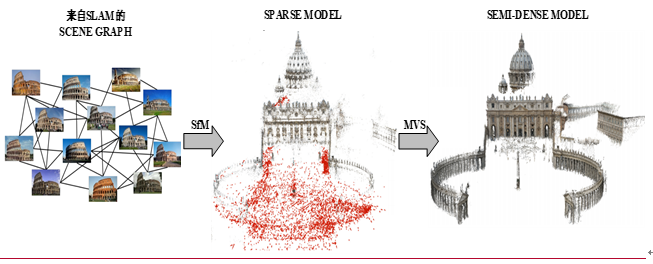
\includegraphics[height=4.5cm]{3d_constr_pipeline_sfm_mvs.png}
  \caption{离线3D重建技术流程图}
  \label{fig:3d_constr_pipeline_sfm_mvs}
\end{figure}
\section{本章小结}
\label{sec:3.4}
本章研究了基于传统三维重建系统的实现流程,包括数据的采集,特征的提取匹配,SfM过程获取稀疏点云,MVS过程获取稠密点云等,只需要向系统中输入围绕堆体拍摄的连续图像,即可得到关于堆体场景的点云模型。

本章揭示了传统三维重建存在的问题,包括系统耗时以及点云模型结果精确度不高等问题,提出了基于传统三维重建的改进方法,即结合实时运行的SLAM系统得出的粗糙scene graph及点云环境地图结果,为三维重建提供先验信息,结合三维重建全局大尺度地图及运动轨迹的优化目标,使用鲁棒性更高的特征描述算子,进行全局BA优化,得到更加精确的全局稀疏地图和运动轨迹。

通过本章基于改进后方法获取到的堆体点云模型,可以提供给基于纯视觉方法测量堆体体积。因此,本章需要获取到高精度的堆体点云结果,以减小后续体积测量误差。